\documentclass[12pt]{article}

\usepackage[utf8x]{inputenc} % Включаем поддержку UTF8  
\usepackage[russian]{babel}  % Включаем пакет для поддержки русского языка  
\usepackage{hyperref}        % Для гиперссылок

% Математика
\usepackage{amsmath}         % В т.ч. для матриц
\usepackage{amssymb}

% Прога
\usepackage{etoolbox}
\usepackage{listings}

% Цвета
\usepackage{xcolor}

% Картинки
\usepackage{graphicx}
\graphicspath{ {./images/} }

\newtheorem{property}{Свойство}
\newtheorem{consequence}{Следствие}[property]

\newcommand{\qedsymbol}{\rule{2mm}{2mm}}

\begin{document}

\thispagestyle{empty}
\begin{center}
\textbf{ПРАВИТЕЛЬСТВО РОССИЙСКОЙ ФЕДЕРАЦИИ}

\vspace{5ex}
	
\textbf{Федеральное государственное автономное образовательное учреждение \\ высшего образования \\ <<Национальный исследовательский университет \\ <<Высшая школа экономики>>}
\end{center}
\vspace{5ex}

\begin{center}
    Московский институт электроники и математики им. А.Н. Тихонова  
    
    \vspace{5ex}
    
    Департамент прикладной математики
    
    \vspace{10ex}
    \textbf{Отчёт \\ по лабораторной работе №8 \\ по курсу <<Алгоритмизация и программирование>>}
	\vspace{7ex}

\end{center}

\begin{center} 
\begin{tabular}{| p{0.3\linewidth}| p{0.3\linewidth}| p{0.3\linewidth}|}
 \hline	
ФИО студента & Номер группы & Дата \\  \hline
 & & \\  
Вязов Глеб \newline Дмитриевич & БПМ-231 & 10.02.2024\\  
 & & \\  \hline		
\end{tabular}
\end{center}

\begin{center}
	\vspace{3ex}
	
	\vfill
   
   \normalsize
    
	\textbf{Москва, 2023}
\end{center}

\newpage

%---------------------------------------------------------------------------------

\section*{Задание (вариант №7)}
\begin{enumerate}
\item Данные должны храниться в бинарном файле.
\item Каждая операция с данными базы должна быть реализована как функция или набор
функций.
\item Выбор и запуск требуемого режима (действия) осуществляется через меню.
\item Реализовать следующие функции обработки данных:
\begin{enumerate}
\item добавление записи в файл;
\item удаление заданной записи из файла по порядковому номеру записи;
\item поиск записей по заданному пользователем (любому) полю структуры;
\item редактирование (изменение) заданной записи;
\item вывод на экран содержимого файла в табличном виде.
\end{enumerate}
\item Структуру (в соответствии с вариантом) определять в отдельном заголовочном файле. С
помощью директив условной компиляции определить два способа ввода исходных данных в
файл: пользователем с потока ввода и из заранее заполненного массива.
\end{enumerate}

\textbf{Данные об олимпийской сборной команде:} ФИО спортсмена, возраст, рост, вес, вид спорта,
спортивное звание.

\newpage

%---------------------------------------------------------------------------------

\section*{Решение}\addcontentsline{toc}{section}{Решение}

\lstset{ %
texcl=true,%
language=C,                 % выбор языка для подсветки
basicstyle=\small\sffamily, % размер и начертание шрифта для подсветки кода
numbers=left,               % где поставить нумерацию строк (слева\справа)
numberstyle=\tiny,           % размер шрифта для номеров строк
stepnumber=1,                   % размер шага между двумя номерами строк
numbersep=5pt,                % как далеко отстоят номера строк от подсвечиваемого кода
backgroundcolor=\color{white}, % цвет фона подсветки - используем \usepackage{color}
showspaces=false,            % показывать или нет пробелы специальными отступами
showstringspaces=false,      % показывать или нет пробелы в строках
showtabs=false,             % показывать или нет табуляцию в строках
frame=single,              % рисовать рамку вокруг кода
tabsize=3,                 % размер табуляции по умолчанию равен 2 пробелам
captionpos=t,              % позиция заголовка вверху [t] или внизу [b] 
breaklines=true,           % автоматически переносить строки (да\нет)
breakatwhitespace=false, % переносить строки только если есть пробел
escapeinside={\%*}{*)},   % если нужно добавить комментарии в коде
inputencoding=utf8x,
extendedchars=\true
}

\begin{lstlisting}[label=structs.h, caption=structs.h]
#ifndef HW8_STRUCTS_H
#define HW8_STRUCTS_H

# define N 50

struct Sportsmen {
    char fio[N];  // ФИО
    int age;      // Возраст
    int height;   // Рост
    int weight;   // Вес
    char type[N]; // Вид спорта
    char rank[N]; // Спотртивное звание
};

void printSportsmen(struct Sportsmen sportsmen);

void findSportsmensByFIO(char fio[]);
void findSportsmensByAge(int age);
void findSportsmensByHeight(int height);
void findSportsmensByWeight(int weight);
void findSportsmensByType(char type[]);
void findSportsmensByRank(char rank[]);

#endif
\end{lstlisting} 

\newpage

\begin{lstlisting}[label=repository.c, caption=repository.c]
#include <stdio.h>
#include <string.h>
#include "structs.h"

#define FILE_NAME "hw8/data.bin"

// Поиск спортсменов по ФИО
void findSportsmensByFIO(char fio[]) {
    FILE *fp;
    fp = fopen(FILE_NAME, "r");
    struct Sportsmen s;
    int result = 1;

    while (!feof(fp)) {
        if (fread(&s, sizeof(s), 1, fp) > 0 && strcmp(fio, s.fio) == 0) {
            printSportsmen(s);
            result = 0;
        }
    }
    printf("\n");
    fclose(fp);

    if (result) {
        printf("Таких спортсменов нет!");
    }
}

// Поиск спортсменов по возрасту
void findSportsmensByAge(int age) {
    FILE *fp;
    fp = fopen(FILE_NAME, "r");
    struct Sportsmen s;
    int result = 1;

    while (!feof(fp)) {
        if (fread(&s, sizeof(s), 1, fp) > 0 && s.age == age) {
            printSportsmen(s);
            result = 0;
        }
    }
    printf("\n");
    fclose(fp);

    if (result) {
        printf("Таких спортсменов нет!");
    }
}

// Поиск спортсменов по росту
void findSportsmensByHeight(int height) {
    FILE *fp;
    fp = fopen(FILE_NAME, "r");
    struct Sportsmen s;
    int result = 1;

    while (!feof(fp)) {
        if (fread(&s, sizeof(s), 1, fp) > 0 && s.height == height) {
            printSportsmen(s);
            result = 0;
        }
    }
    printf("\n");
    fclose(fp);

    if (result) {
        printf("Таких спортсменов нет!");
    }
}

// Поиск спортсменов по весу
void findSportsmensByWeight(int weight) {
    FILE *fp;
    fp = fopen(FILE_NAME, "r");
    struct Sportsmen s;
    int result = 1;

    while (!feof(fp)) {
        if (fread(&s, sizeof(s), 1, fp) > 0 && s.weight == weight) {
            printSportsmen(s);
            result = 0;
        }
    }
    printf("\n");
    fclose(fp);

    if (result) {
        printf("Таких спортсменов нет!");
    }
}

// Поиск спортсменов по виду спорта
void findSportsmensByType(char type[]) {
    FILE *fp;
    fp = fopen(FILE_NAME, "r");
    struct Sportsmen s;
    int result = 1;

    while (!feof(fp)) {
        if (fread(&s, sizeof(s), 1, fp) > 0 && strcmp(type, s.type) == 0) {
            printSportsmen(s);
            result = 0;
        }
    }
    printf("\n");
    fclose(fp);

    if (result) {
        printf("Таких спортсменов нет!");
    }
}

// Поиск спортсменов по спортивному званию
void findSportsmensByRank(char rank[]) {
    FILE *fp;
    fp = fopen(FILE_NAME, "r");
    struct Sportsmen s;
    int result = 1;

    while (!feof(fp)) {
        if (fread(&s, sizeof(s), 1, fp) > 0 && strcmp(rank, s.rank) == 0) {
            printSportsmen(s);
            result = 0;
        }
    }
    printf("\n");
    fclose(fp);

    if (result) {
        printf("Таких спортсменов нет!");
    }
}
\end{lstlisting} 

\newpage

\begin{lstlisting}[label=structs.h, caption=hw8.c]
#include <stdio.h>
#include <windows.h>
#include <unistd.h>
#include "repository.c"

#define option 0

void scanfSportsmen(struct Sportsmen *s);
void addSportsmen(struct Sportsmen sportsmen);
void deleteSportsmen(int index);
void updateSportsmen(int index, struct Sportsmen sportsmen);
void printFile();
void filter();
int getMaxHeight();

int main() {
    // Меняем кодировку на UTF-8, чтобы можно было писать на русском
    SetConsoleOutputCP(CP_UTF8);
    // Ввод переменных. Дружественный интерфейс
    printf("Выполнил задание: Вязов Глеб. Группа: БПМ231\n");

    FILE *fp;
    fp = fopen(FILE_NAME, "r");

    // Если файл не создан, то создаем
    if (fp == NULL) {
        printf("Такого файла нет!\n");
        fp = fopen(FILE_NAME, "wb");
        printf("Создан файл с именем %s!\n", FILE_NAME);
    }
    fclose(fp);

    // Заполняем данные из массива
#if option==0
    struct Sportsmen sportsmens[] = {
            {"Вязов Глеб", 17, 164, 56, "Шахматы", "3 разряд"},
            {"Иван Иванов Иванович", 23, 180, 84, "Тяжелая атлетика", "КМС"},
            {"Павел Артемьев", 43, 200, 120, "Паурлифтинг", "МСМК"},
            {"Емельяненко Федор", 35, 180, 80, "ММА", "ЧМ"},
            {"Арнольд Шварцнегер", 100, 180, 100, "Бодибилдинг", "ЧМ"},
            {"Луговой Александр", 40, 180, 56, "Пауэрлифтинг", "МСМК"},
            {"Сарычев Кирилл", 40, 200, 140, "Жим лежа", "МСМК"},
            {"Джулиус Мэддокс", 35, 170, 150, "Жим лежа", "ЧМ"},
            {"Сарычев Кирилл", 40, 200, 140, "Становая тяга", "МСМК"},
            {"Тайсон Майк", 57, 178, 80, "Бокс", "ЧМ"},
            };
    for (int i=0; i<10; i++) {
        addSportsmen(sportsmens[i]);
    }
    // Заполняем данные из консоли
#else
    int count;
    struct Sportsmen sp;
    printf("Количество записей: ");
    scanf("%d", &count);
    for (int i=0; i<count; i++) {
        scanfSportsmen(&sp);
        addSportsmen(sp);
    }
#endif
    printf("Вывести содержимое файла -- 0\n"
                  "Добавить запись в конец  -- 1\n"
                  "Удалить запись           -- 2\n"
                  "Обновить запись          -- 3\n"
                  "Поиск по полю структуры  -- 4\n"
                  "Завершить программу      -- 5\n");

    struct Sportsmen s;
    int index, flag = 1;

    printf("\nСамые высокие спортсмены:\n");
    int maxHeight = getMaxHeight();
    findSportsmensByHeight(maxHeight);

    while (flag) {
        int command;
        scanf("%d", &command);

        switch (command) {
            case 0: printFile(); break;
            case 1:
                scanfSportsmen(&s);
                addSportsmen(s);
                break;
            case 2:
                printf("\nВведите индекс: ");
                scanf("%d", &index);
                deleteSportsmen(index);
                break;
            case 3:
                scanfSportsmen(&s);
                printf("\nВведите индекс: ");
                scanf("%d", &index);
                updateSportsmen(index, s);
                break;
            case 4:
                filter();
                break;
            case 5:
                flag = 0;
        }
    }

    return 0;
}

// Функция вызывает функцию поиска в зависимости от введенных значений
void filter() {
    int command2, param2;
    char param1[50];

    printf("Введите номер поля:");
    scanf("%d", &command2);
    switch (command2) {
        case 0:
            printf("\nВведите ФИО: ");
            scanf("%s", param1);
            findSportsmensByFIO(param1);
            break;
        case 1:
            printf("\nВведите возраст: ");
            scanf("%d", &param2);
            findSportsmensByAge(param2);
            break;
        case 2:
            printf("\nВведите рост: ");
            scanf("%d", &param2);
            findSportsmensByHeight(param2);
            break;
        case 3:
            printf("\nВведите вес: ");
            scanf("%d", &param2);
            findSportsmensByWeight(param2);
            break;
        case 4:
            printf("\nВведите вид спорта: ");
            scanf("%s", param1);
            findSportsmensByType(param1);
            break;
        case 5:
            printf("\nВведите спортивное звание: ");
            scanf("%s", param1);
            findSportsmensByRank(param1);
            break;
    }
}

// Считать данные спортсмена через консоль
void scanfSportsmen(struct Sportsmen *s) {
    printf("\nВведите ФИО: ");
    fflush(stdin);
    gets(s->fio);
    printf("\nВведите возраст: ");
    scanf("%d", &s->age);
    printf("\nВведите рост: ");
    scanf("%d", &s->height);
    printf("\nВведите вес: ");
    scanf("%d", &s->weight);
    printf("\nВведите вид спорта: ");
    fflush(stdin);
    gets(s->type);
    printf("\nВведите спортивное звание: ");
    gets(s->rank);
}

// Вывод спортсмена в консоль
void printSportsmen(struct Sportsmen sportsmen) {
    printf("%s, %d, %d, %d, %s, %s\n", sportsmen.fio, sportsmen.age, sportsmen.height, sportsmen.weight,
           sportsmen.type, sportsmen.rank);
}

// Добавление спортсмена в конец файла
void addSportsmen(struct Sportsmen sportsmen) {
    FILE *fp;
    fp = fopen(FILE_NAME, "a");
    fwrite(&sportsmen, sizeof(sportsmen), 1, fp);
    fclose(fp);
}

// Удаление спортсмена по индексу. Индексация с нуля
void deleteSportsmen(int index) {
    FILE *fp;
    fp = fopen(FILE_NAME, "r+");

    // Считаем количество записей в файле
    fseek(fp, 0L, SEEK_END);
    int len = ftell(fp) / sizeof(struct Sportsmen);

    // Перемещаем курсор на index+1 позицию
    fseek(fp, (index+1)*sizeof(struct Sportsmen), SEEK_SET);
    struct Sportsmen s;

    for (int i=index; i<len-1; i++) {
        fread(&s, sizeof(s), 1, fp);              // cursor = i+1
        fseek(fp, i*sizeof(struct Sportsmen), SEEK_SET);     // cursor = i
        fwrite(&s, sizeof(struct Sportsmen), 1, fp);      // cursor = i --> cursor = i+1
        fseek(fp, (i+2)*sizeof(struct Sportsmen), SEEK_SET); // cursor = i+2
    }

    // Уменьшаем размер файла
    _chsize( fileno(fp), (len-1)*sizeof(struct Sportsmen));
    fclose(fp);
}

// Вместо спортсмена на index позиции ставиться sportsmen
// Нумерация с нуля
void updateSportsmen(int index, struct Sportsmen sportsmen) {
    FILE *fp;
    fp = fopen(FILE_NAME, "r+");

    fseek(fp, index*sizeof(struct Sportsmen), SEEK_SET);
    fwrite(&sportsmen, sizeof(struct Sportsmen), 1, fp);

    fclose(fp);
}

// Вывод содержимого файла в консоль
void printFile() {
    FILE *fp;
    fp = fopen(FILE_NAME, "r");
    struct Sportsmen s;

    while (!feof(fp)) {
        if (fread(&s, sizeof(s), 1, fp) > 0) {
            printSportsmen(s);
        }
    }
    printf("\n");
    fclose(fp);
}

// Найти самых высоких спортсменов
int getMaxHeight() {
    FILE *fp;
    fp = fopen(FILE_NAME, "r");
    struct Sportsmen s;
    int maxHeight = 0;

    while (!feof(fp)) {
        if (fread(&s, sizeof(s), 1, fp) > 0) {
            if (maxHeight <= s.height) {
                maxHeight = s.height;
            }
        }
    }
    return maxHeight;
}
\end{lstlisting} 

\newpage

%---------------------------------------------------------------------------------

\section*{Тестирование}


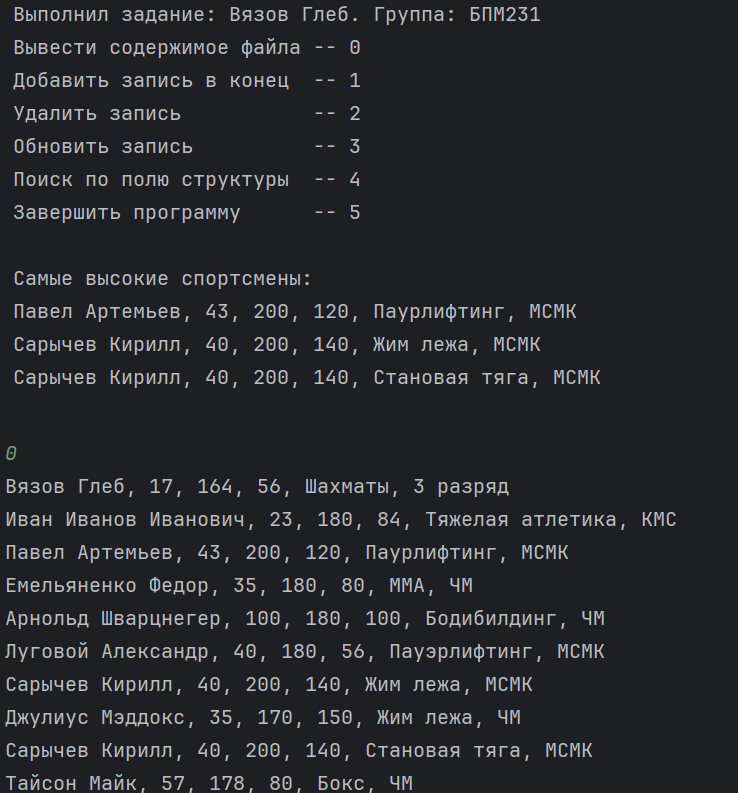
\includegraphics[scale=0.8]{img1}

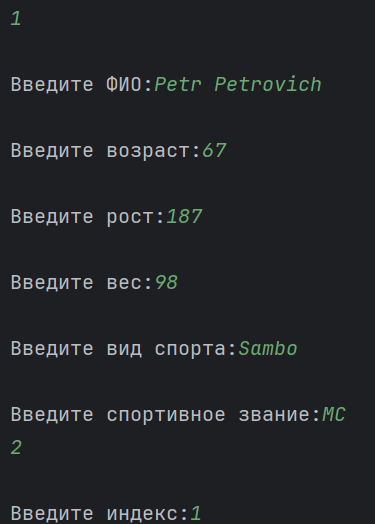
\includegraphics[scale=0.8]{img2}

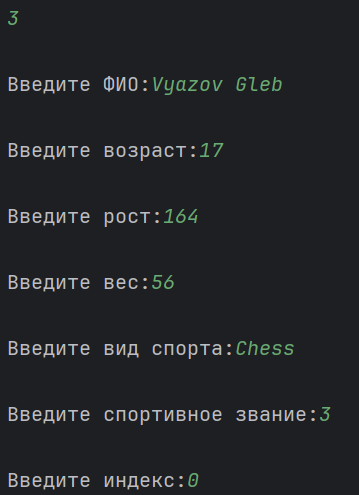
\includegraphics[scale=0.8]{img3}

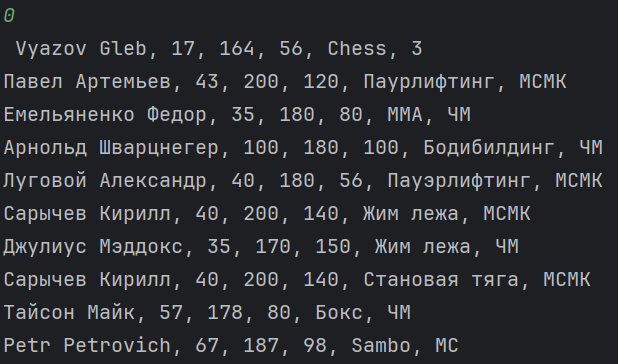
\includegraphics[scale=0.8]{img4}

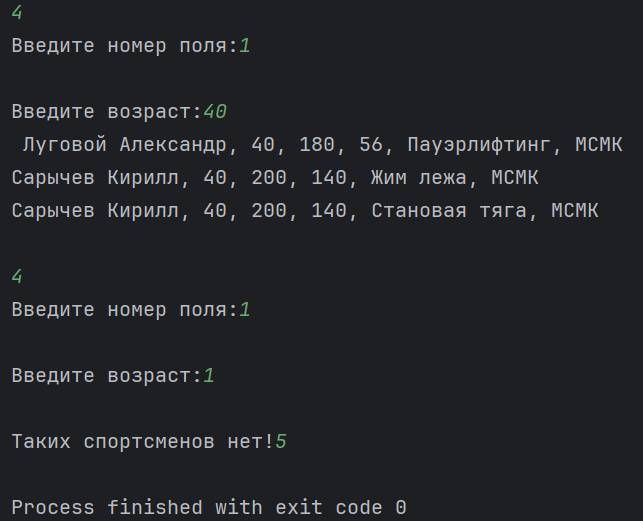
\includegraphics[scale=0.8]{img5}



\end{document}
